\documentclass[11pt]{article}
\usepackage{amsmath}
\usepackage{amssymb}
\usepackage{graphicx}
\usepackage{float}
\usepackage{fancyhdr}
\usepackage{enumerate}
\usepackage{titlesec}
\usepackage[colorlinks=true,urlcolor=blue]{hyperref}

\titlespacing{\subsubsection}{0pt}{0pt}{0pt}

% No page numbers
%\pagenumbering{gobble}

% INFORMATION SHEET (DO NOT EDIT THIS PART) ---------------------------------------------
\newcommand{\addinformationsheet}{
\clearpage
\thispagestyle{empty}
\begin{center}
\LARGE{\bf \textsf{Information sheet\\CS224W: Machine Learning with Graphs}} \\*[4ex]
\end{center}
\vfill
\textbf{Assignment Submission } Fill in and include this information sheet with each of your assignments.  This page should be the last page of your submission.  Assignments are due at 11:59pm and are always due on a Thursday.  All students (SCPD and non-SCPD) must submit their homework via GradeScope (\url{http://www.gradescope.com}). Students can typeset or scan their homework. Make sure that you answer each (sub-)question on a separate page. That is, one answer per page regardless of the answer length. Students also need to upload their code on Gradescope. Put all the code for a single question into a single file and upload it.  
\\
\\
\textbf{Late Homework Policy } Each student will have a total of {\em two} late periods. {\em Homework are due on Thursdays at 11:59pm PT and one late period expires on the following Monday at 11:59pm PT}.  Only one late period may be used for an assignment.  Any homework received after 11:59pm PT on the Monday following the homework due date will receive no credit.  Once these late periods are exhausted, any assignments turned in late will receive no credit.
\\
\\
\textbf{Honor Code } We strongly encourage students to form study groups. Students may discuss and work on homework problems in groups. However, each student must write down their solutions independently, i.e., each student must understand the solution well enough in order to reconstruct it by him/herself.  Students should clearly mention the names of all the other students who were part of their discussion group. Using code or solutions obtained from the web (GitHub/Google/previous year's solutions etc.) is considered an honor code violation. We check all the submissions for plagiarism. We take the honor code very seriously and expect students to do the same. 
\vfill
}

% MARGINS (DO NOT EDIT) ---------------------------------------------
\oddsidemargin  0.25in \evensidemargin 0.25in \topmargin -0.5in
\headheight 0in \headsep 0.1in
\textwidth  6.5in \textheight 9in
\parskip 1.25ex  \parindent 0ex \footskip 20pt
% ---------------------------------------------------------------------------------

% HEADER (DO NOT EDIT) -----------------------------------------------
\newcommand{\problemnumber}{0}
\newcommand{\myname}{name}
\newfont{\myfont}{cmssbx10 scaled 1000}
\pagestyle{fancy}
\fancyhead{}
\fancyhead[L]{\myfont Question \problemnumber, Homework 1, CS224W}
%\fancyhead[R]{\bssnine \myname}
\newcommand{\newquestion}[1]{
\clearpage % page break and flush floats
\renewcommand{\problemnumber}{#1} % set problem number for header
\phantom{}  % Put something on the page so it shows
}
% ---------------------------------------------------------------------------------


% BEGIN HOMEWORK HERE
\begin{document}

% Question 1.1
\newquestion{1.1}

The log-log degree distribution plot is shown as belows. We can see that
\begin{itemize}
    \item The Small World Network has the most narrow plot comparing to other two networks.
    \item Erdos Renyi Network is more similar with Collaboration Network, which means from the degree distribution perspective, Erdos Renyi models the real networks better.
    \item Compared to random graph networks, the degree distribution of Collaboration Network is more wider.
    \item It has more long-tail nodes which has large degree and small degree.
\end{itemize}
\begin{figure}[H]
    \centering
    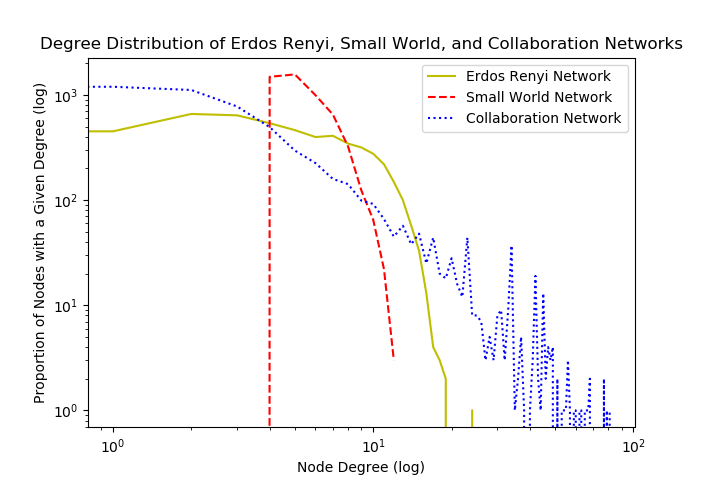
\includegraphics[width=0.80\textwidth]{pics/deg_distribution.png}
\end{figure}

% Question 1.2
\newquestion{1.2}

The average clustering coefficient for each network:
\begin{itemize}
    \item Clustering Coefficient for Erdos Renyi Network: 0.000802
    \item Clustering Coefficient for Small World Network: 0.149388
    \item Clustering Coefficient for Collaboration Network: 0.264818
\end{itemize}
We can see that Collaboration Network has the largest average clustering coefficient. \\\\
Since in real life, authors are likely to establish collaboration with those who have collaborated with their collaborators, so the local structure of this subgraph tends to be dense, which results in a larger average clustering coefficient.

% Question 2.1
\newquestion{2.1}

% Question 2.2
\newquestion{2.2}

% Question 2.3a
\newquestion{2.3a}

% Question 2.3b
\newquestion{2.3b}

% Question 3.1
\newquestion{3.1}

% Question 3.2
\newquestion{3.2}

% Question 3.3
\newquestion{3.3}

% Question 3.3
\newquestion{3.4}

% Question 4.1
\newquestion{4.1}

% Question 4.2
\newquestion{4.2}

% Question 4.3
\newquestion{4.3}


% Information sheet
% Fill out the information below (this should be the last page of your assignment)
\addinformationsheet
\vfill

{\Large
    \textbf{Your name:} \hrulefill  % Put your name here
    \\
    \\
    \textbf{Email:} \underline{\hspace*{7cm}}  % Put your e-mail here
    \textbf{SUID:} \hrulefill  % Put your student ID here
    \\*[2ex]
}
Discussion Group: \hrulefill   % List your study group here
\\
\vfill\vfill
I acknowledge and accept the Honor Code.\\*[3ex]
\bigskip
\textit{(Signed)}
\hrulefill   % Replace this line with your initials
\vfill






\end{document}